%% 
%% Copyright 2019-2024 Elsevier Ltd
%% 
%% This file is part of the 'CAS Bundle'.
%% --------------------------------------

\documentclass[a4paper,fleqn]{cas-dc}

\usepackage[authoryear,longnamesfirst]{natbib}
\usepackage{amsmath,amssymb,mathtools,booktabs,graphicx}
\usepackage{bm}
\usepackage{xspace}
\usepackage{etoolbox}
\usepackage{placeins}

%%% Author macros
\def\tsc#1{\csdef{#1}{\textsc{\lowercase{#1}}\xspace}}
\tsc{WGM}
\tsc{QE}
%%%

\newtheorem{theorem}{Theorem}
\newtheorem{proposition}{Proposition}
\newtheorem{corollary}{Corollary}
\newdefinition{remark}{Remark}
\newproof{proof}{Proof}


\setcounter{topnumber}{5}
\setcounter{totalnumber}{10}
\renewcommand{\topfraction}{0.9}
\renewcommand{\textfraction}{0.05}

\begin{document}
	
	\let\WriteBookmarks\relax
	\def\floatpagepagefraction{1}
	\def\textpagefraction{.001}
	
	\shorttitle{Hybrid probability estimation via log-odds offset stacking}
	\shortauthors{H. Malata}
	
	\title[mode=title]{Hybrid probability estimation via log-odds offset stacking with hierarchical calibration}
	
	\tnotemark[1]
\tnotetext[1]{This letter presents the mathematical formulation of a hybrid probability estimator derived from a larger empirical study on macroprudential early-warning modelling in SADC banking systems. The empirical analysis will be reported separately.}
	
\author[1]{Hedson Malata}[orcid=0009-0006-4029-712X]

\cormark[1]

\ead{hedson.malata@northrise.net}

\credit{Conceptualization; Methodology; Formal analysis; Software; Data curation; Visualization; Writing -- original draft; Writing -- review and editing.}
	
	\affiliation[1]{
		organization={Northrise Business School, Northrise University},
		city={Ndola},
		country={Zambia}
	}
	
	
	\cortext[1]{Corresponding author}
	
	\begin{abstract}
		This paper introduces a hybrid probability estimator designed for short and heterogeneous panels. 
		The method combines a structural time-series prior with a discriminative machine-learning predictor through an offset formulation on the log-odds scale. The resulting hybrid probabilities are calibrated using a global post-hoc mapping and, when justified by out-of-sample performance, a guarded country-specific isotonic adjustment.
		
		The proposed estimation problem is strictly convex and therefore admits a unique solution. The hybrid construction preserves ranking whenever the offset weight is positive, ensuring that calibration improves probability reliability without distorting discrimination.
		
		A compact numerical illustration based on annual prudential aggregates for six SADC banking systems shows that the calibrated hybrid improves pooled out-of-sample Brier score and log-loss relative to both structural and machine-learning baselines while maintaining useful discrimination.
		
		The framework is general and applicable to a wide class of small-panel forecasting problems where reliable probabilistic predictions are required.
	\end{abstract}
	
	\begin{highlights}
		\item Hybrid probability estimation via offset stacking of structural and machine-learning logits.
		\item Strict convexity of the penalized likelihood guarantees a unique estimator.
		\item Hierarchical calibration improves reliability in small heterogeneous panels.
	\end{highlights}
	
	\begin{keywords}
		Calibrated probabilities \sep forecast combination \sep log-odds stacking \sep small panels \sep macroprudential early-warning
	\end{keywords}
	
	\maketitle
	
	\section{Introduction}
	Probabilistic early-warning systems are widely used in finance, engineering
	reliability, and public risk monitoring to detect adverse events before they
	materialize. In such settings, predictive models are expected not only to rank
	observations correctly but also to provide reliable probability estimates. The
	quality of probabilistic forecasts is therefore evaluated using proper scoring
	rules and calibration diagnostics. Poorly calibrated probabilities may lead to
	systematically biased risk assessments even when the underlying classifier
	achieves good discrimination performance.
	
	A large literature has proposed post-processing methods for improving
	probability calibration. Techniques such as Platt scaling, isotonic
	regression, and related calibration procedures adjust the outputs of a
	predictive model in order to better align predicted probabilities with
	observed event frequencies
	\citep{Platt1999,ZadroznyElkan2002,NiculescuMizilCaruana2005,GuoEtAl2017,KullEtAl2017}.
	Forecast combination methods provide another perspective by aggregating
	predictions from multiple models to improve predictive accuracy
	\citep{BatesGranger1969,Clemen1989}.
	
	The hybrid formulation proposed in this paper differs from both approaches by
	integrating structural and machine-learning probabilities directly within a
	single estimator defined on the log-odds scale. In this formulation, the
	structural probability acts as a prior offset, while the machine-learning
	predictor contributes incremental predictive evidence through a weighted
	log-odds adjustment.
	In many macro-financial applications, early-warning systems are estimated using panel data with limited time dimensions and heterogeneous cross-sectional units. Traditional crisis-prediction studies rely on indicator-based or econometric models to identify leading signals of financial distress \citep{Kaminsky1998leading,Demirguc1998determinants,BussiereFratzscher2006}. Structural time-series models offer interpretable probabilistic forecasts by exploiting temporal smoothing and latent state dynamics \citep{Harvey1990,DurbinKoopman2012}. However, such models may be too restrictive to capture nonlinear relationships present in modern financial datasets. Conversely, purely machine-learning approaches can capture complex interactions but often suffer from instability and poor calibration when applied to small samples.
	
	A natural solution is to combine forecasts from structurally motivated models and flexible predictive learners. The theory of forecast combination shows that appropriately weighted ensembles can improve predictive accuracy relative to individual models \citep{BatesGranger1969,Clemen1989}. In the context of probabilistic prediction, combining forecasts on the log-odds scale provides a convenient framework that preserves interpretability while allowing additional information to enter the model incrementally.
	
	Motivated by these considerations, this paper proposes a hybrid probability estimator that combines a structural prior probability with a discriminative machine-learning score through an offset formulation on the log-odds scale. In the proposed construction, the structural probability acts as a baseline prior, while the machine-learning predictor contributes incremental evidence through a weighted log-odds adjustment. This formulation yields a simple yet flexible hybrid estimator that can subsequently be calibrated using standard monotone calibration methods.
	
	We establish two theoretical properties of the estimator. First, the penalized likelihood used to estimate the hybrid parameters is strictly convex, implying the existence of a unique minimizer. Second, the hybrid log-odds mapping preserves ranking whenever the offset weight is positive, ensuring that monotone calibration procedures improve probability reliability without altering discrimination.
	
	A compact numerical illustration based on annual prudential aggregates for several Southern African banking systems demonstrates that the calibrated hybrid improves pooled out-of-sample Brier score and log-loss relative to both structural and machine-learning baselines. The proposed framework therefore provides a simple and mathematically transparent approach to combining structural modelling, machine learning, and probability calibration in small heterogeneous panels.
	
	
	\section{Hybrid model and calibration}
	
	We construct a hybrid probabilistic predictor by combining a structurally motivated probability estimate with a discriminative machine-learning forecast. The approach can be viewed as a probabilistic analogue of forecast combination, where multiple predictive sources are aggregated to improve predictive accuracy \citep{BatesGranger1969,Clemen1989}. The combination is implemented on the log-odds scale, which provides a natural representation for probability adjustments.
	
	Let $y_t\in\{0,1\}$ denote a binary outcome and let $x_t\in\mathbb{R}^p$ denote the associated predictor vector.
	
	Two base probability estimates are constructed.
	
	\paragraph{Structural prior.}
	
	A smoothed latent mean is obtained through an exponentially weighted recursion
	\begin{equation}
		m_t=\alpha y_t+(1-\alpha)m_{t-1},\qquad \alpha\in(0,1).
	\end{equation}
	
	To stabilize the estimate in short samples, shrinkage toward the training prevalence $\bar y$ yields the structural probability
	
	\begin{equation}
		p_t^{\mathrm{U}}=\lambda_t m_{t-1}+(1-\lambda_t)\bar y,
	\end{equation}
	
	where $\lambda_t\in[0,1]$ controls the effective local sample weight.
	
	\paragraph{Discriminative probability.}
	
	A logistic learner produces the machine-learning probability
	
	\begin{equation}
		p_t^{\mathrm{M}}=\sigma(\beta_0+\beta^\top x_t), \qquad
		\sigma(z)=\frac{1}{1+e^{-z}}.
	\end{equation}
	
	\paragraph{Hybrid log-odds stack.}
	
	Let $\ell(p)=\log\frac{p}{1-p}$ denote the logit map. The hybrid predictor is defined as
	
	\begin{equation}
		\ell(p_t^{\mathrm{H}})
		=
		a+w\bigl(\ell(p_t^{\mathrm{M}})-\ell(p_t^{\mathrm{U}})\bigr)
		+\ell(p_t^{\mathrm{U}}).
	\end{equation}
	
	Equivalently,
	
	\begin{equation}
		p_t^{\mathrm{H}}
		=
		\sigma
		\left(
		a+w(\ell(p_t^{\mathrm{M}})-\ell(p_t^{\mathrm{U}}))
		+\ell(p_t^{\mathrm{U}})
		\right).
	\end{equation}
	
	In this formulation the structural probability $p_t^{\mathrm{U}}$ acts as a prior offset, while the parameter $w$ measures the incremental contribution of the machine-learning predictor. When $w=0$ the hybrid reduces to the structural model, whereas positive values of $w$ allow the discriminative predictor to adjust the prior probability through log-odds evidence.
	
	\paragraph{Calibration.}
	
	Raw hybrid probabilities are mapped to calibrated probabilities
	
	\[
	\tilde p_t = C(p_t^{\mathrm{H}})
	\]
	
	using a monotone calibration map $C$. Common choices include Platt scaling \citep{Platt1999}, isotonic regression \citep{ZadroznyElkan2002,NiculescuMizilCaruana2005}, and beta calibration \citep{KullEtAl2017}.
	
	For heterogeneous panels we optionally use a hierarchical blend
	
	\begin{equation}
		\tilde p_{c,t}
		=
		(1-\alpha_c)C_{\mathrm{glob}}(p_{c,t}^{\mathrm{H}})
		+
		\alpha_c C_c(p_{c,t}^{\mathrm{H}}),
	\end{equation}
	
	where $C_{\mathrm{glob}}$ denotes a global calibration map and $C_c$ denotes a country-specific calibration function. The local map is accepted only if it improves out-of-sample loss by a predefined margin, thereby preventing overfitting in small samples.
\section{Mathematical properties}

We now establish several basic properties of the hybrid estimator, including its interpretation as a log-odds shrinkage estimator, the convexity of the estimation problem, and invariance of ranking under calibration.

The parameters $(a,w)$ are estimated by minimizing the penalized negative log-likelihood

\begin{equation}
	L(a,w)
	=
	-\sum_{t=1}^{N}
	\Big[
	y_t\log p_t^{\mathrm{H}}
	+
	(1-y_t)\log(1-p_t^{\mathrm{H}})
	\Big]
	+
	\gamma w^2,
\end{equation}

where $\gamma>0$ is a regularization parameter.

\begin{proposition}[Log-odds shrinkage interpretation]
	
	The hybrid logit defined by
	
	\[
	\ell(p_t^{\mathrm{H}})
	=
	a+w(\ell(p_t^{\mathrm{M}})-\ell(p_t^{\mathrm{U}}))+\ell(p_t^{\mathrm{U}})
	\]
	
	can be rewritten as
	
	\[
	\ell(p_t^{\mathrm{H}})
	=
	(1-w)\ell(p_t^{\mathrm{U}})+w\ell(p_t^{\mathrm{M}})+a .
	\]
	
	Thus the hybrid predictor corresponds to a shrinkage estimator on the log-odds scale that interpolates between the structural and machine-learning logits.
	
\end{proposition}

\begin{proof}
	
	Expanding the hybrid logit expression gives
	
	\[
	\ell(p_t^{\mathrm{H}})
	=
	a+w\ell(p_t^{\mathrm{M}})-w\ell(p_t^{\mathrm{U}})+\ell(p_t^{\mathrm{U}}).
	\]
	
	Collecting terms yields
	
	\[
	\ell(p_t^{\mathrm{H}})
	=
	(1-w)\ell(p_t^{\mathrm{U}})+w\ell(p_t^{\mathrm{M}})+a,
	\]
	
	which shows that the hybrid logit is an affine combination of the structural and machine-learning logits.
	
\end{proof}



\begin{corollary}[Convex log-odds combination]
	
	If the weight satisfies $w\in[0,1]$, the hybrid logit
	
	\[
	\ell(p_t^{\mathrm{H}})
	=
	(1-w)\ell(p_t^{\mathrm{U}})+w\ell(p_t^{\mathrm{M}})+a
	\]
	
	corresponds to a convex combination of the structural and machine-learning logits up to an affine shift. Consequently, the hybrid predictor belongs to the class of forecast-combination estimators on the log-odds scale.
	
\end{corollary}

\begin{proof}
	
	For $w\in[0,1]$, the coefficients $(1-w)$ and $w$ are nonnegative and sum to one. Hence the hybrid logit is a convex combination of $\ell(p_t^{\mathrm{U}})$ and $\ell(p_t^{\mathrm{M}})$, up to the additive intercept $a$, which does not affect convexity of the combination.
	
\end{proof}


\begin{theorem}
	
	The objective function $L(a,w)$ is strictly convex in $(a,w)\in\mathbb{R}^2$. Consequently the hybrid estimator admits a unique minimizer.
	
\end{theorem}

\begin{proof}
	
	Define
	
	\[
	\eta_t(a,w)
	=
	a+w\bigl(\ell(p_t^{\mathrm{M}})-\ell(p_t^{\mathrm{U}})\bigr)
	+\ell(p_t^{\mathrm{U}}).
	\]
	
	The Bernoulli negative log-likelihood is
	
	\[
	\phi(\eta;y)
	=
	-y\log\sigma(\eta)-(1-y)\log(1-\sigma(\eta)).
	\]
	
	Its second derivative is
	
	\[
	\frac{\partial^2 \phi}{\partial \eta^2}
	=
	\sigma(\eta)(1-\sigma(\eta))>0.
	\]
	
	Hence $\phi$ is convex in $\eta$. Since $\eta_t(a,w)$ is affine in $(a,w)$, convexity is preserved under affine composition. The ridge penalty $\gamma w^2$ is strictly convex, implying that the total objective $L(a,w)$ is strictly convex and therefore possesses a unique minimizer.
	
\end{proof}

\begin{proposition}
	
	Assume $w>0$. If $p_i^{\mathrm{M}}>p_j^{\mathrm{M}}$ and $p_i^{\mathrm{U}}=p_j^{\mathrm{U}}$, then $p_i^{\mathrm{H}}>p_j^{\mathrm{H}}$.
	
\end{proposition}

\begin{proof}
	
	The hybrid logit is affine and strictly increasing in the quantity $\ell(p_t^{\mathrm{M}})-\ell(p_t^{\mathrm{U}})$ whenever $w>0$. Since the logistic map $\sigma(z)$ is strictly increasing, the ordering of probabilities is preserved.
	
\end{proof}

\begin{remark}
	
	Because Platt scaling and isotonic regression are monotone transformations, calibration procedures improve probability reliability while preserving the ranking induced by the hybrid predictor.
	
\end{remark}

\begin{proposition}[Calibration invariance]
	
	Let $p_t^{\mathrm{H}}$ denote hybrid probabilities and let $\tilde p_t = C(p_t^{\mathrm{H}})$ where $C:[0,1]\to[0,1]$ is a strictly increasing calibration map.
	
	Then the ranking induced by the hybrid probabilities is preserved, i.e.
	
	\[
	p_i^{\mathrm{H}} > p_j^{\mathrm{H}}
	\quad\Rightarrow\quad
	\tilde p_i > \tilde p_j .
	\]
	
\end{proposition}

\begin{proof}
	
	Since $C$ is strictly increasing on $[0,1]$, it preserves order. Therefore for any $i,j$ such that $p_i^{\mathrm{H}}>p_j^{\mathrm{H}}$ we have
	
	\[
	C(p_i^{\mathrm{H}}) > C(p_j^{\mathrm{H}}).
	\]
	
	Thus calibration improves probability reliability while leaving the discrimination ranking unchanged.
	
\end{proof}
\section{Compact numerical illustration}

We illustrate the hybrid estimator using the annual SADC country--year panel
employed in the larger empirical study. The panel covers Botswana, Malawi,
Namibia, South Africa, Tanzania, and Zambia over the period 2004--2024.

The predictor set consists of standard prudential indicators commonly used in
macroprudential early-warning models, including the equity-to-assets ratio,
return on assets, asset growth, and short lagged balance-sheet variables.
Model evaluation is conducted using an out-of-sample forecasting procedure in
which parameters are estimated on historical observations and predictions are
generated for subsequent periods. This design mimics real-time monitoring
settings in which early-warning indicators must be evaluated on previously
unseen data.

Table~\ref{tbl1} reports pooled out-of-sample performance for the competing
estimators. The hierarchical-calibrated hybrid achieves the best overall
performance across all reported scoring rules. In particular, it attains a
Brier score of $0.215$, log-loss of $0.621$, AUC of $0.633$, and average
precision of $0.632$, outperforming both the structural baseline and the
standalone machine-learning predictor.


\begin{table}[t]
	\caption{Pooled out-of-sample performance in the SADC illustration.}
	\label{tbl1}
	\begin{tabular*}{\tblwidth}{@{\extracolsep{\fill}}lcccc@{}}
		\toprule
		Model & Brier & Log-loss & AUC & AP \\
		\midrule
		Hybrid (hierarchical calibration) & \textbf{0.215} & \textbf{0.621} & \textbf{0.633} & \textbf{0.632} \\
		Hybrid (global calibration) & 0.223 & 0.639 & 0.618 & 0.552 \\
		Structural baseline & 0.243 & 0.721 & 0.500 & -- \\
		ML baseline & 0.267 & 0.836 & 0.503 & -- \\
		\bottomrule
	\end{tabular*}
\end{table}

Figure~\ref{fig:roc} compares receiver operating characteristic curves for the
competing estimators. The hybrid predictor retains discrimination performance
comparable to the structural baseline while substantially outperforming the
standalone machine-learning model.

\begin{figure}[t]
	\centering
	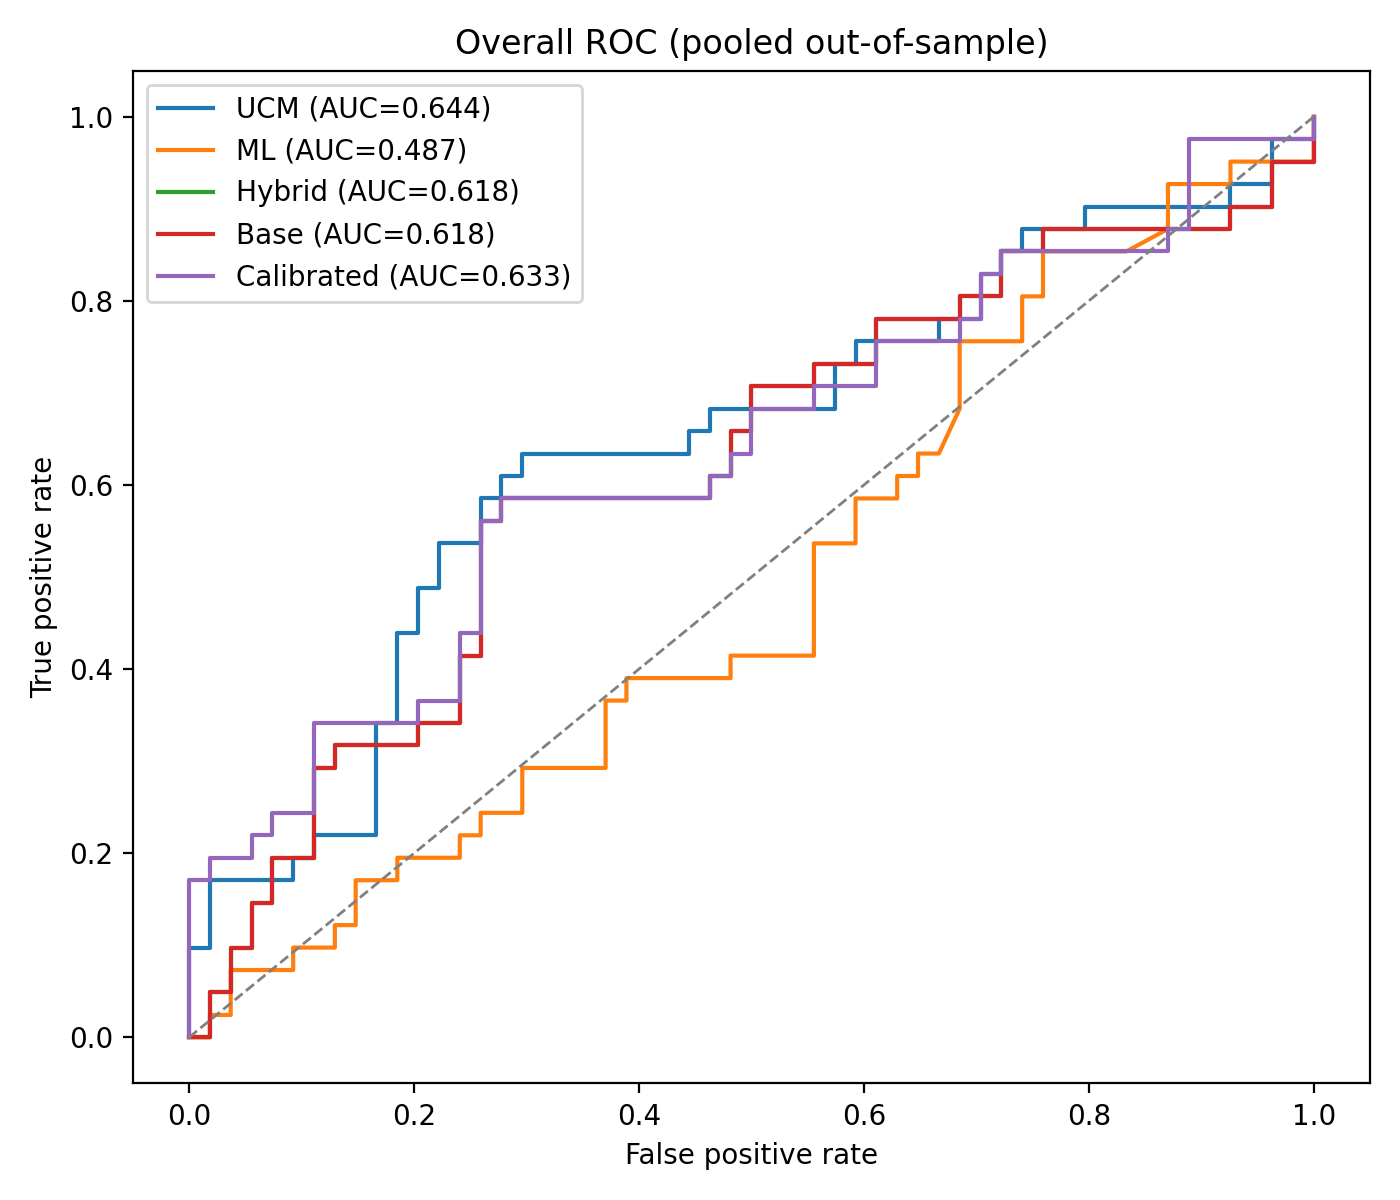
\includegraphics[width=0.85\linewidth]{01_overall_roc.png}
	\caption{Receiver operating characteristic curves for the structural (UCM),
		machine-learning (ML), hybrid, and calibrated hybrid estimators evaluated
		out-of-sample on the pooled panel.}
	\label{fig:roc}
\end{figure}

Figure~\ref{fig:calibration} evaluates probability reliability. The reliability
diagram compares predicted probabilities with observed event frequencies. The
uncalibrated hybrid probabilities exhibit moderate miscalibration, while the
post-hoc calibration mapping moves predictions closer to the ideal diagonal,
improving probability reliability without altering ranking.

\begin{figure}[t]
	\centering
	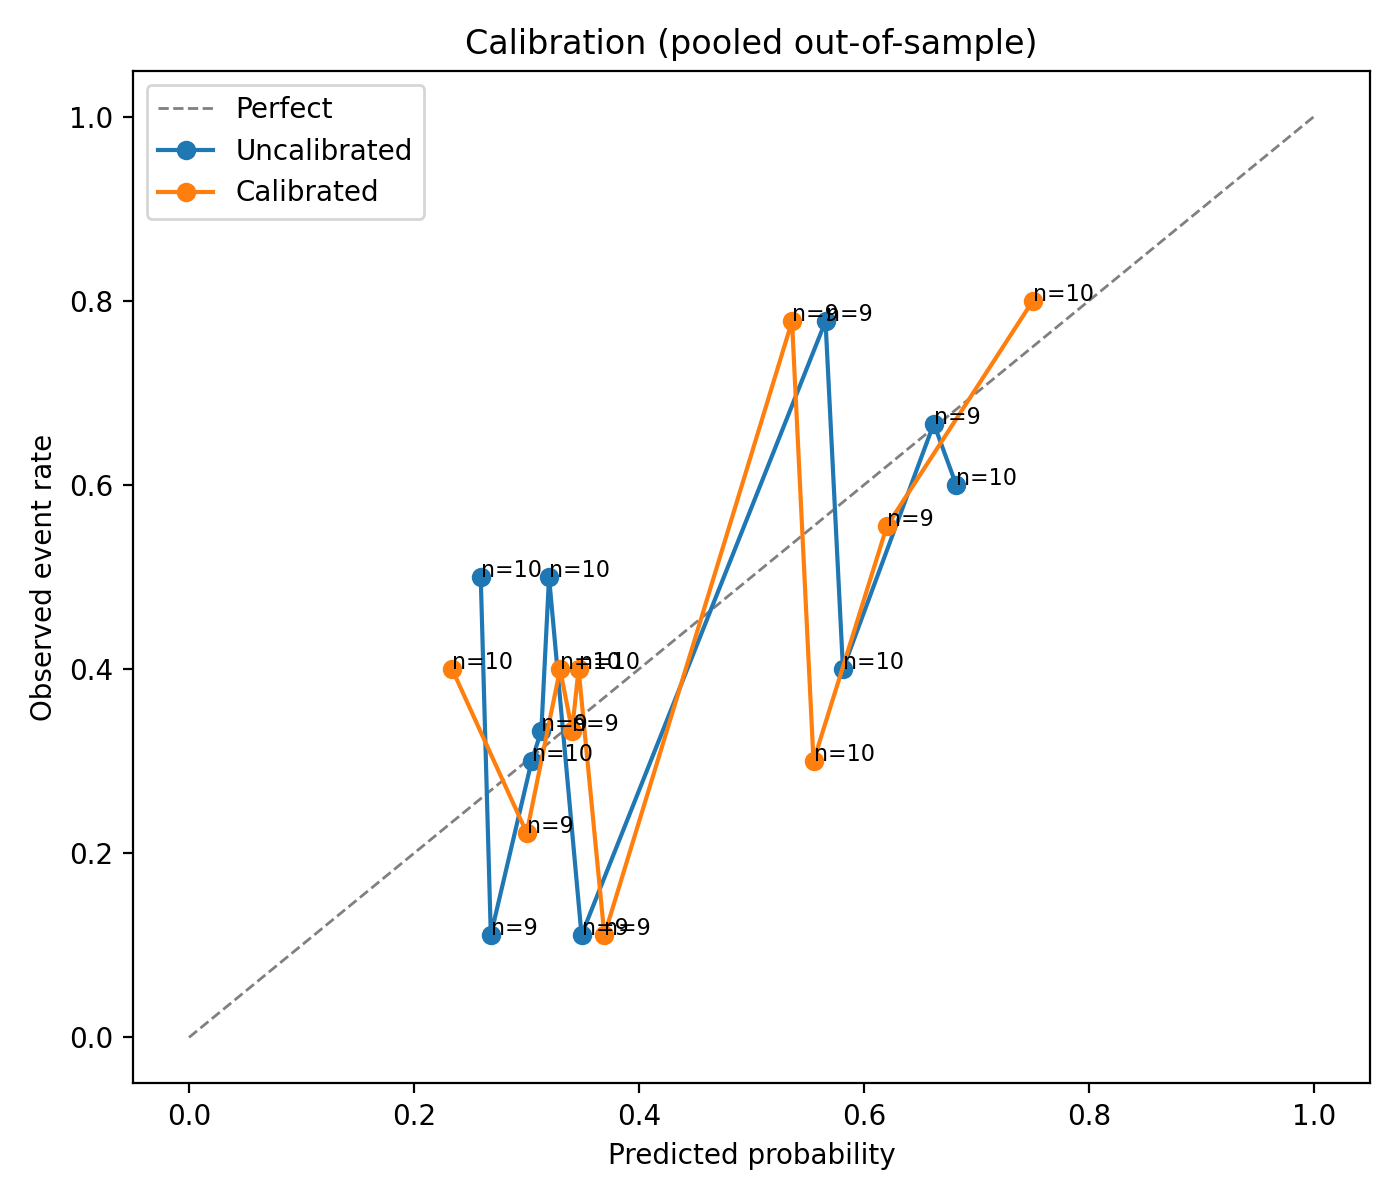
\includegraphics[width=0.85\linewidth]{03_overall_calibration.png}
	\caption{Calibration curves comparing uncalibrated and calibrated hybrid
		probabilities. The dashed line denotes perfect calibration.}
	\label{fig:calibration}
\end{figure}

Because early-warning applications often involve class imbalance,
Figure~\ref{fig:pr} reports precision--recall curves. The calibrated hybrid
achieves the highest average precision, confirming that the hybrid estimator
improves predictive performance in rare-event settings.

The hybrid estimator was also evaluated across alternative calibration schemes and prediction horizons. While performance varies across specifications, the hybrid construction consistently improves probability reliability relative to purely structural and purely machine-learning baselines. These findings indicate that the offset formulation provides a stable mechanism for combining structural information with flexible predictive models, improving both probability reliability and discrimination in short heterogeneous panels.

\begin{figure}[t]
	\centering
	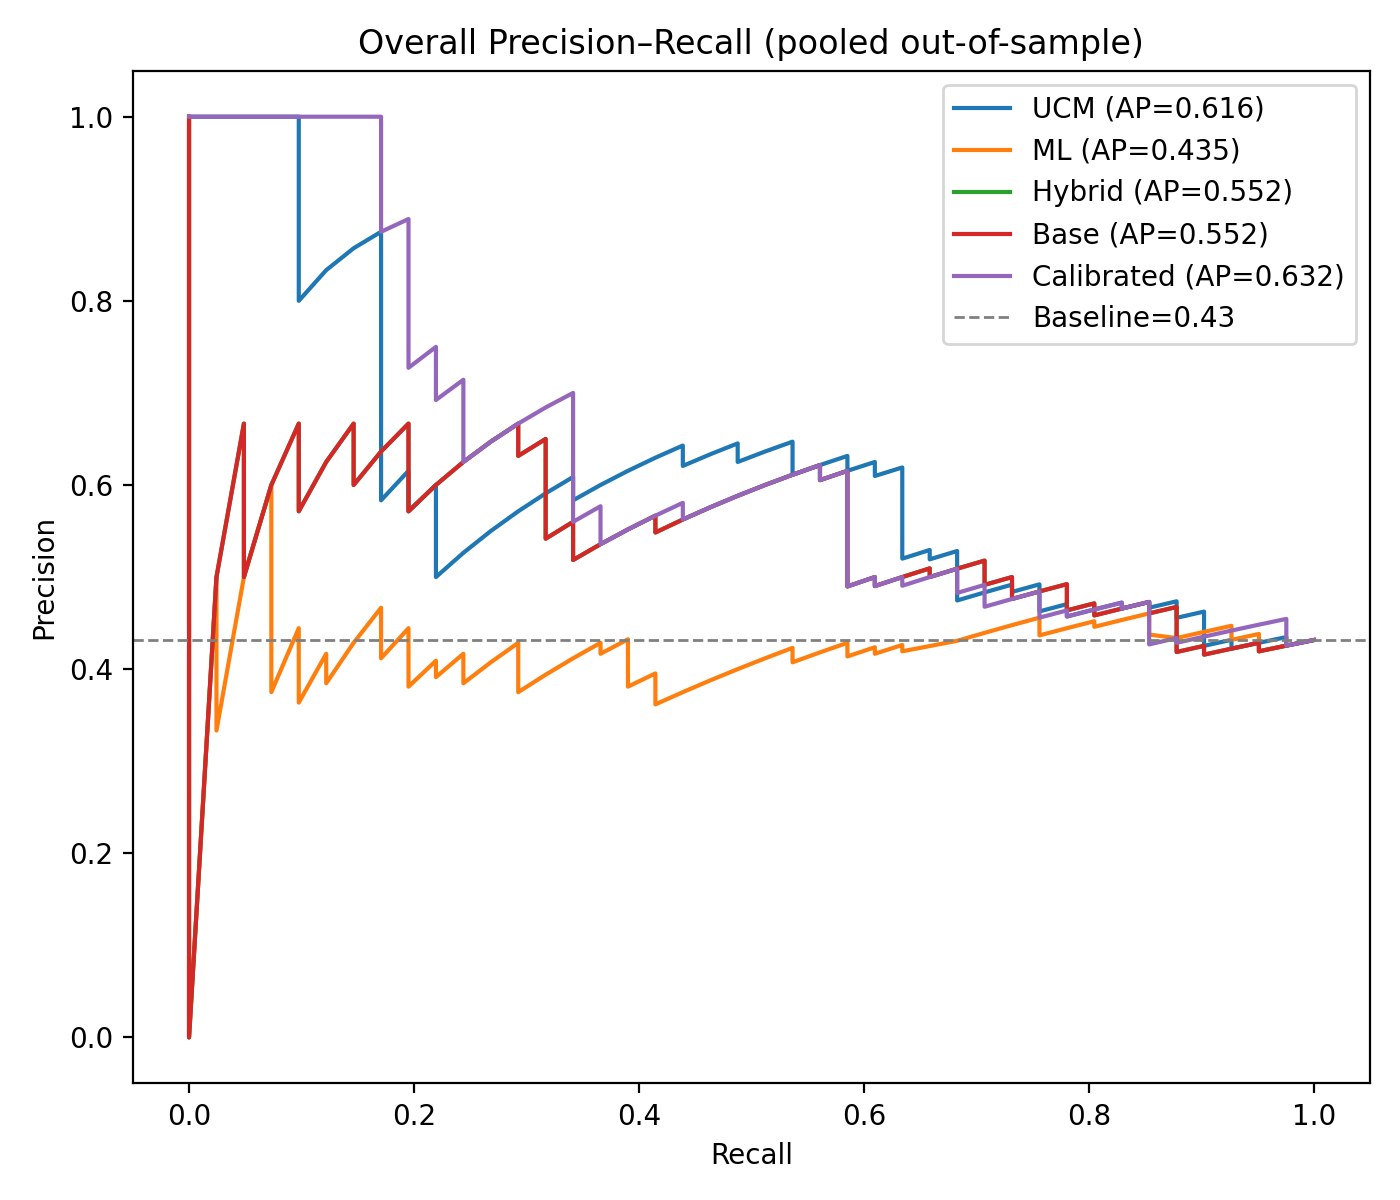
\includegraphics[width=0.85\linewidth]{02_overall_pr.png}
	\caption{Precision--recall curves for the competing models evaluated
		out-of-sample on the pooled panel.}
	\label{fig:pr}
\end{figure}
	
\FloatBarrier

\section{Discussion and conclusion}

This letter isolates the core methodological component of a broader empirical framework: a hybrid probability estimator that combines structural information with discriminative machine-learning predictions through an offset formulation on the log-odds scale. The resulting hybrid predictor can be interpreted as a shrinkage estimator that interpolates between a structural prior and a data-driven learner.

The offset representation preserves interpretability because the structural probability remains explicit in the model formulation. At the same time, the machine-learning component contributes incremental predictive information through a weighted log-odds adjustment. The resulting estimation problem is strictly convex, ensuring the existence and uniqueness of the hybrid estimator, while post-hoc monotone calibration improves probability reliability without affecting discrimination.

The empirical illustration based on the SADC country-year panel demonstrates that the hybrid construction can improve probabilistic forecasting performance in short and heterogeneous panels. In particular, the hierarchical calibration scheme enhances probability reliability while retaining useful ranking performance relative to both structural and purely machine-learning baselines.

Although motivated by macroprudential early-warning modelling, the proposed framework is broadly applicable to forecasting problems where reliable probability estimates are required but data are limited or heterogeneous. Potential applications include medical risk prediction, reliability analysis of engineering systems, and demand forecasting in public services.
The proposed framework also has several limitations. The relative contribution of the structural and machine-learning components depends on the estimated offset weight, which may be sensitive to very small samples or extreme class imbalance. In addition, the empirical illustration relies on a relatively short panel of country-level observations. These limitations motivate further evaluation of the method in larger datasets and alternative application domains.

Future work may extend the framework by incorporating richer structural state-space models, developing theoretical bounds for calibration error, and generalizing the hybrid formulation to multi-horizon or sequential forecasting settings.
	\printcredits
	
	\FloatBarrier
	\bibliographystyle{cas-model2-names}
	\bibliography{cas-refs}
	
\end{document}